\documentclass[a4paper, french]{article}

%% Language and font encodings
\usepackage{babel}
\usepackage[utf8]{inputenc}
\usepackage[T1]{fontenc}

%% Sets page size and margins
\usepackage[%
a4paper,top=3cm,bottom=2cm,left=2.5cm,right=2.5cm,%
marginparwidth=1.75cm]{geometry}
\usepackage{multicol}
\usepackage{parskip}


%% Useful packages
\usepackage{amsmath}
\usepackage{amsfonts}
\usepackage{graphicx}
\graphicspath{ {images/} }
\usepackage[colorinlistoftodos]{todonotes}
\usepackage[colorlinks=true, allcolors=black]{hyperref}
\usepackage{float}
\usepackage{listings}

%% verbatim listings
\usepackage{xparse}
\lstset{basicstyle=\ttfamily}
\NewDocumentCommand{\cword}{v}{%
    \texttt{#1}%
}

\title{compte rendu -- projet bioinformatique --\\%
Analyse statistique d'une famille de Prot\'eines}
\author{Ben Kirane Malik}

\begin{document}
\maketitle
\setlength{\parskip}{0.1in}
\setlength{\parindent}{15pt}
\begin{abstract}
    Il nous est proposé d'analyser une famille de prot\'eines
    pr\'ealablement s\'equenc\'ee. Nous rendrons compte de comment
    exploiter des outils statistiques et probabilistes pour
    analyser ces séquences protéiques et en d\'eduire des propri\'et\'es
    de conservation au sein de la famille, d'appartenance \`a la famille
    et finalement pour esquisser une corr\'elation entre
    l'alignement des prot\'eines et des mesures spatiales.
    %conduites sur cette famille.
\end{abstract}

\section{Pr\'eliminaire}

Dans l'int\'egralit\'e des analyses nous ferons r\'ef\'erence \`a une
unique famille de prot\'eines, $D_{train}$.
Nous avons acc\`es \`a $M=5643$ prot\'eines toutes de cette famille.
%
Chaque prot\'eine est d\'ecrite par une s\'equence et
ces s\'equences, forment l'\emph{alignement}
que nous \'etudions par la suite.  Une prot\'eine de l'alignement se
pr\'esente comme une suite d'acide amin\'es (il y en a 20)
avec \'eventuellement des trous dans la s\'equence.
%
% peut etre histograme acides amines dans l'alignement ?
% si il y a encore de la place
%

Il s'agit dans un premier temps de lire l'alignement propos\'e
(fichier \cword{data/Dtrain.txt}) au format FASTA.
Chaque ligne non pr\'ec\'ed\'ee du caract\`ere '\cword{>}'
d\'ecrit une prot\'eine de la famille $D_{train}$ sur l'alphabet
\begin{equation*}
    \mathcal{A}=\{\cword{A},\cword{C},\cword{D},\cword{E},\cword{F},\cword{G},
    \cword{H},\cword{I},\cword{K},\cword{L},\cword{M},\cword{N},\cword{P},
\cword{Q},\cword{R},\cword{S},\cword{T},\cword{V},\cword{W},\cword{Y},\cword{-}\}
\end{equation*}
pour les $L=48$ positions possibles de l'alignement que nous souhaitons \'etudier.

Les impl\'ementations des analyses du projet sont r\'ealis\'es en
\cword{python} (version \cword{3.6}). 
Ici, pour la lecture de l'alignement le code se trouve
dans le module \cword{data} (\cword{src/data.py}) o\`u on peux utiliser
la m\'ethode \cword{read_fasta(filename)} pour lire les lignes qui nous
int\'eressent dans \cword{data/Dtrain.txt} et avoir la liste des s\'equences
de l'alignement.

\`A pr\'esent que nous avons acc\`es \`a l'alignement, nous souhaiterions
savoir ce qui caract\'erise les s\'equences qui le constituent et notamment
comment mettre en \'evidence les positions caract\'eristiques fortes de
l'alignement.

\section{Conservation des positions et caract\`ere de l'alignement}

L'alignement se repr\'esente avec une matrice $M$ lignes et $L$ colonnes.
Les lignes de cette matrice correspondent aux s\'equences et les colonnes
aux positions de l'alignement.

\subsection{\'Evaluation du caract\`ere de l'alignement}
On s'int\'eresse au nombre d'occurences d'%
un acide amin\'e $a\in\mathcal{A}$ \`a la  position $i$, $0\leq i\leq L-1$.
On note $n_i(a)$ cette quantit\'e. En supposant que les positions sont
ind\'ependantes on souhaite d\'eterminer $\omega$ tel que
\begin{equation*}
    P(a_0\ldots a_{L-1}|\omega)=
    \prod_{i=0}^{L-1} \underbrace{P(a_i|\omega)}_{\omega_i(a_i)}
\end{equation*}
il s'agit de la matrice commun\'ement appel\'ee
``position-specific weight matrix'' ou PSWM.

Il est donc question d'estimer la PSWM $\omega$ avec les $n_i(a)$ et en
utilisant un estimateur de fr\'equence corrig\'e avec un pseudo-compteur
de valeur 1, donc
\begin{equation*}
    \omega_i(a) = \frac{n_i(a) + 1}{M+|\mathcal{A}|}.
    \label{eq:estimateur_pswm}
\end{equation*}

Le calcul d'estimation de la PSWM est impl\'ement\'e dans le module
\cword{pswm} (\cword{src/pswm.py}) par\break
\cword{estimate_pswm(data)} avec \cword{data} la liste des
s\'equences lues depuis \cword{data/Dtrain.txt}.

Pour caract\'eriser notre famille, on va chercher les position les plus
conserv\'ees. Pour cela, nous mesurons la quantit\'e d'information relative
\`a une position
% remarque: interruption du fonctionnement de la proteine
\begin{equation*}
    S_i = \log_2(q) +
    \sum_{a\in\matchal{A}} \omega_i(a)
    \cdot
    \log_2\left(\omega_i(a)\right)
\end{equation*}
c'est l'entropie de Shannon l\'eg\`erement corrig\'e. L'impl\'ementation
de ce calcul est r\'ealis\'e par\break
\cword{shannon_pswm(i, pswm)} dans
\cword{pswm} et \cword{real2()} du m\^eme module r\'ealise toute la
proc\'edure jusqu'au trac\'e de l'entropie relative en fonction de la
position (F\textsc{igure} \ref{fig:shannon_relative}).

\begin{figure}[h]
\begin{center}
    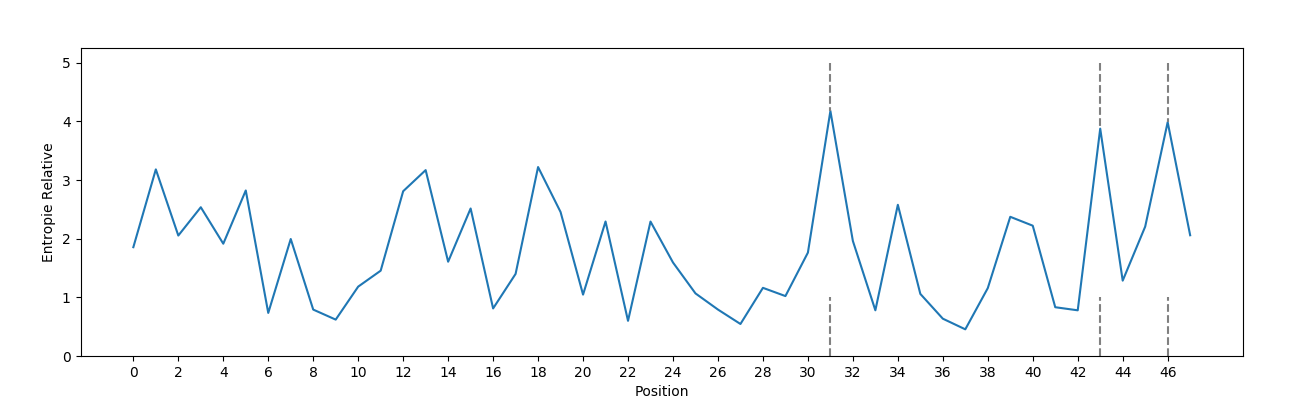
\includegraphics[width=14cm]{images/shannon_relative}
    \caption{Quantit\'e d'information aux positions de l'alignement}
    \label{fig:shannon_relative}
\end{center}
\end{figure}

L'entropie maximale est presque significativement atteinte aux positions
31, 46 et 43. Cela signifie que ces positions ont un r\^ole important
pour la famille de prot\'eines. Ces positions sont tr\`es fortement conserv\'ees
et si il advenait qu'elles soient modif\'ees, cela pertuberait fortement
la fonction biologique premi\`ere de la prot\'eine.

Par la suite nous allons examiner si la PSWM nous permet d'identifier
si d'autres s\'equences sont aussi dans la famille.

\subsection{Crit\'ere d'appartenance \`a la famille de prot\'eines}

\'Etant donn\'e une s\'equence quelconque $b_0\ldots b_{N-1}$, $N\geq L$,
nous souhaitons savoir si un fragment de cette s\'equence appartient
\`a la famille de prot\'eines. Supposons d'abord $N=L$.

On peut estimer un mod\`ele qui ne soit pas sp\'ecifiique aux positions,
c'est \`a dire tel que
\begin{equation*}
    P(b_0\ldots b_{L-1}) = \prod_{i=0}^{L-1} f^{(0)}(b_i)
\end{equation*}
et
\begin{equation*}
    \forall{b\in \mathcal{A}},
    f^{(0)}(b)=\frac{1}{L}\sum_{i=0}^{L-1}\omega_i(b).
\end{equation*}
Il s'agit d'un mod\`ele nul.
Nous comparons alors ce mod\`ele nul avec le mod\`ele PSWM \'evalu\'e sur
la famille de prot\'eines $D_{train}$. Pour cela, nous \'evaluons la quantit\'e
\newcommand{\lodd}{\mathpzc{l}}
\begin{equation*}
    \lodd(b_0\ldots b_{L-1}) = \log_2
    \frac{P(b_0\ldots b_{L-1}|\omega)}{P(b_0\ldots b_{L-1})}
\end{equation*}

\newpage
ou encore
\begin{equation*}
    \lodd(b_0\ldots b_{L-1}) =
    \sum_{i=0}^{L-1} \left(\log_2 \omega_i(b_i) - \log_2 f^{(0)}(b_i)\right).
\end{equation*}
Si $\lodd(b_0\ldots b_{L-1})>0$, on saura que la s\'equence $b$
est plus probable d'appara\^itre dans le mod\`ele PSWM que le mod\`ele nul
et r\'eciproquement si $\lodd(b_0\ldots b_{L-1})<0$, $b$ est peu probable d'appartenir \`a la famille. 
La mesure $\lodd$ est appel\'ee \emph{log-vraissemblance}.

Reprenons maintenant \`a $N\geq L$. Il suffit de faire glisser une fen\^etre
de taille $L$ sur $b$ et de noter pour chaque d\'ecalage la valeur de $\lodd$
sur la fen\^etre.

Nous disposons d'une s\'equence dans \cword{data/testseq.txt} pour laquelle
nous aimerions savoir si une partie appartient \`a la famille de
prot\'eines $D_{train}$.

Dans le module \cword{pswm} (\cword{src/pswm.py}),
\begin{itemize}
    \item \cword{null_model(pswm)} est la m\'ethode qui calcul les
        valeurs $f^{(0)}$  d\'ecrivant le mod\`ele nul,
    \item \cword{log_odds(sequence, pswm, f0)} calcul la log-vraissemblance
        d'une s\'equence,
    \item \cword{sliding_odds(sequences, pswm)} calcul sur l'ensemble des
        fen\^etres possibles les log-vraissemblances.
\end{itemize}
Finalement la fonction \cword{real4()} r\'ealise l'ensemble des manipulations
d\'ecrites jusqu'ici et affiche le trac\'e de la log-vraissemblance en fonction
du d\'ecalage de la fen\^etre glissante
(F\textsc{igure} \ref{fig:log_odds}).

\begin{figure}[h]
    \begin{center}
        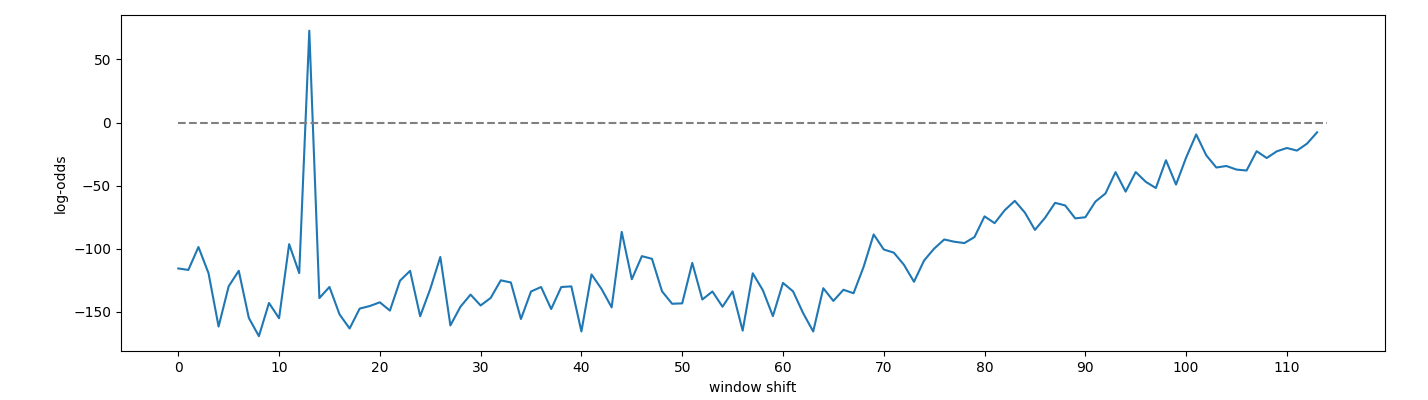
\includegraphics[width=15cm]{images/log_odds}
        \caption{Log-vraissemblances sur la s\'equence test}
        \label{fig:log_odds}
    \end{center}
\end{figure}

Pour la sous-s\'euence $(b_{13}\ldots b_{13+L-1})$ on observe que la
log-vraissemblance est positive, c'est d'ailleurs la seule fen\^etre o\`u
c'est le cas, et par cons\'equent cette sous-s\'equence
appartient tr\`es probablement \`a la famille de prot\'eine que l'on \'etudie.
Il est aussi tr\`es probable que cette sous-s\'equence
ai les m\^emes fonctions biologiques que les prot\'eines
de la famille \'etudi\'e.

\section{Co-\'evolution et corr\'elation avec la structure spatiale}

Nous allons chercher \`a pr\'esent \`a mettre en relation l'information
des s\'equences de l'alignement avec la structure spatiale d'une prot\'eine
repr\'esentative de la famille. Cela dit, nous devons enrichir le mod\`ele
PSWM d\'ecrit avant pour tenir compte de la structure spatiale.

La piste
propos\'ee est d'estimer la co-\'evolution de deux positions. Pour deux
acides amin\'es $a$ et $b$ on souhaite savoir s'ils sont pr\'esents dans la
s\'equence tel que $a$ soit \`a une premi\`ere position donn\'ee et que $b$ soit
\`a une seconde position donn\'ee : il s'agit l\`a d'une co-occurence.

Soit $n_{i,j}(a,b)$ le nombre de s\'equences tel que 
$a$ est \`a la position $i$ et $b$ est \`a la position $j$.
Pour estimer les poids $\omega_{i,j}(a,b)$ associ\'es aux $n_{i,j}(a,b)$,
il faut conserver la relation $\sum_b \omega_{i,j}(a,b)=\omega_i(a)$.

Donc les
\begin{equation*}
    \omega_{i,j}(a,b)=
    \frac{n_{i,j}(a,b) + 1/q}{M+q}
\end{equation*}
sont les composantes de notre mod\`ele enrichit.

Il est possible mainteant de mesurer la quantit\'e d'information mutuelle.
Il s'agit de d\'eterminer \`a quel point deux positions sont corr\'el\'ees.

La quantit\'e d'information mutuelle pour un couple de positions
$(i,j)$ est la quantit\'e
\begin{equation*}
    M_{i,j}=\sum_{a,b\in\mathcal{A}}\omega_{i,j}(a,b)
    \Left[\log_2{\omega_{i,j}(a,b)}-\log_2{\omega_i(a)\omega_j(b)}\Right]
\end{equation*}

Nous disposons d'une table des distances pour des couples de positions
(fichier \cword{data/distances.txt}). On consid\`ere qu'une paire est en
contact si la distance entre ces positions est inf\'erieur \`a 8\r A (0.8nm).
En triant les paires $(i,j)$ par valeurs
d\'ecroissantes de $M_{i,j}$ autrement dit des paires les plus corr\'el\'ees
au moins corr\'el\'ees et en d\'eterminant la fraction de paires en contact
pour chaque tranche de paires selon ce tri, on souhaite d\'eterminer 
une relation entre la structure spatiale et l'information statistique
dont on dispose pour la famille.  
La F\textsc{igure} \ref{fig:contacts} est le trac\'e de cette fraction
en fonction de la taille des tranches (il y a au plus $L^2$ tranches).

\begin{figure}[h]
    \begin{center}
    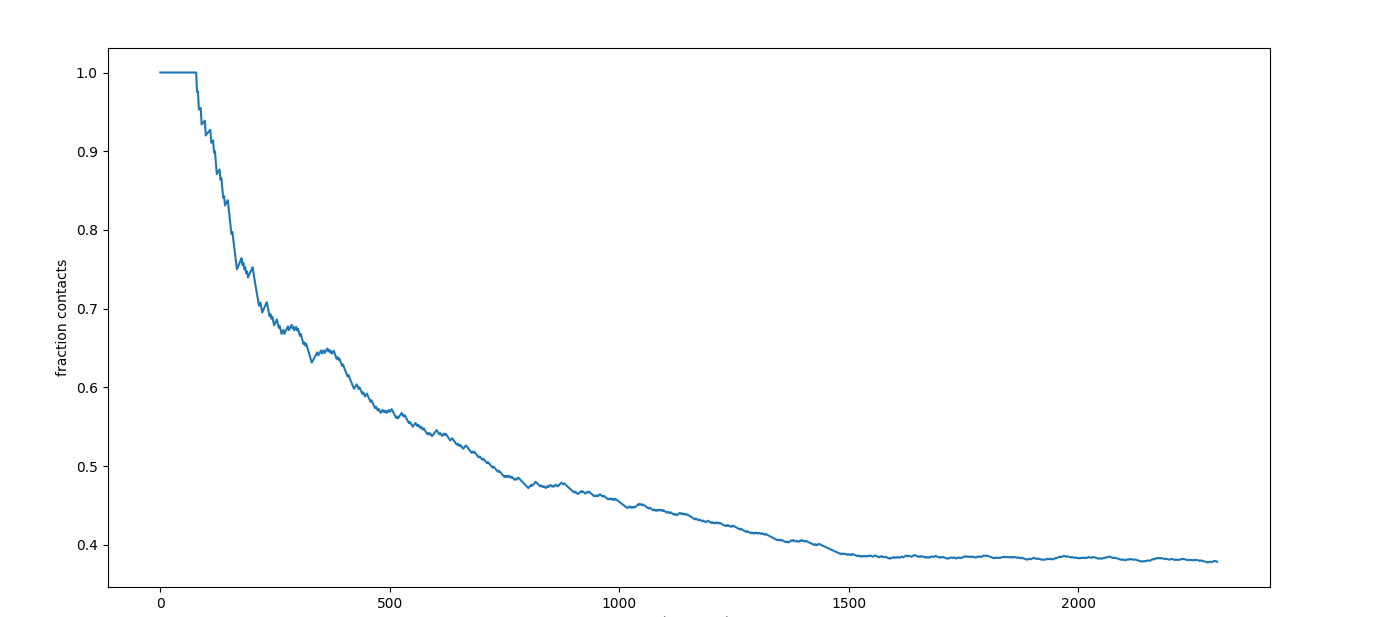
\includegraphics[width=15cm]{images/contacts.png}
    \caption{R\'esidus en contacts (taille de la tranche en abscisse)}
    \label{fig:contacts}
    \end{center}
\end{figure}

Tout le proc\'ed\'e jusqu'\`a la r\'ealisation du trac\'e est impl\'ement\'e
par \cword{real4()} dans le moduel \cword{coev} (\cword{src/coev.py}).
Cette r\'ealisation s'appui sur les fonctions
\begin{itemize}
    \item \cword{estimate_cooc(data)}
        pour le calcul des $\omega_{i,j}(a,b)$;
    \item \cword{mutual_information(cooc, pswm, M)}
        pour le calcul des $M_{i,j}$;
    \item \cword{induced_contacts(mim, distances)}
        qui d\'etermine les fractions des paires en contacts;
\end{itemize}
toutes dans m\^eme module \cword{coev}.

On observe que plus on consid\`ere une tranche de paires fortement 
corr\'el\'ees, plus la fraction de paires en contacts est importante.
D'une part il s'agit d'un r\'esultat obtenu par comptage sur les
s\'equences et d'autre part il s'agit d'une mesure physique et d'une
propri\'et\'e spatiale.
Pour cette famille de prot\'eines, on peut induire la propri\'et\'e
spatiale de contact \`a partir du proc\'ed\'e statistique d\'ecrit
ici, i.e., les paires les plus corr\'el\'ees ont une probabilit\'e
\'elev\'ee d'\^etre en contact.


\hspace{1in}
\paragraph{Conclusion:}
Nous avons mis en \'evidence que les outils statistiques sont des outils
puissant et utiles en biologie. Les proc\'ed\'es d\'ecrits pour
l'analyse de la famille de prot\'eines \'etudi\'ee sont reproductibles si
on dispose d'un alignement d'une autre famille et ils nous permettraient
d'identifier
\vskip 1mm
\begin{itemize}
    \item les positions caract\'erisitiques de la famille qui d\'eterminent
        l'expression de ses fonctions biologiques,
        \vskip 1mm
    \item d'autres s\'equences appartenant probablement \`a la famille et
        \vskip 1mm
    \item des propri\'et\'es spatiales, qui, enrichies par d'autres
        proc\'edures, nous permettrait de
        visualiser en 3D la structure spatiale d'une prot\'eine
        repr\'esentative de la famille.
\end{itemize}

\end{document}
